% !TeX program = xelatex
% Compile twice from this directory; see ../HW2_STA/README.md.
\documentclass[UTF8,a4paper,11pt,fontset=fandol]{ctexart}
\usepackage[left=20mm,right=20mm,top=19mm,bottom=19mm]{geometry}
\usepackage{amsmath,booktabs,array,tabularx,xcolor,listings}
\usepackage{graphicx,float,caption}
\usepackage{xurl}
\usepackage[unicode,colorlinks=true,linkcolor=blue!45!black,urlcolor=blue!45!black]{hyperref}
\graphicspath{{asset/}}
\definecolor{reportblue}{HTML}{25465F}
\hypersetup{pdftitle={HW2 STA - 2300012831},pdfauthor={Tongbin Zhao}}
\ctexset{section={format=\Large\bfseries\color{reportblue},beforeskip=1em,afterskip=0.6em},
  subsection={format=\normalsize\bfseries,beforeskip=0.8em,afterskip=0.4em}}
\setlength{\parindent}{2em}
\setlength{\parskip}{0.25em}
\setlength{\tabcolsep}{5pt}
\setlength{\emergencystretch}{2em}
\renewcommand{\arraystretch}{1.18}
\newcolumntype{P}[1]{>{\raggedright\arraybackslash}p{#1}}
\newcommand{\code}[1]{\texttt{\detokenize{#1}}}
\newcommand{\AT}{\operatorname{AT}}
\newcommand{\RAT}{\operatorname{RAT}}
\newcommand{\slack}{\operatorname{slack}}
\captionsetup{font=small,labelfont=bf,skip=5pt}
\lstdefinestyle{script}{language=Python,basicstyle=\ttfamily\small,
  keywordstyle=\color{blue!60!black},commentstyle=\color{green!35!black},
  stringstyle=\color{red!45!black},numbers=left,numberstyle=\tiny\color{gray},
  numbersep=6pt,breaklines=true,breakatwhitespace=false,
  columns=fullflexible,keepspaces=true,showstringspaces=false,
  frame=single,rulecolor=\color{gray!40},xleftmargin=1.7em,
  aboveskip=0.6em,belowskip=0.6em,tabsize=4}

\begin{document}
\pagestyle{plain}
\begin{center}
  {\LARGE\bfseries HW2 实验报告}\par
  \vspace{0.2em}
  {\large\color{reportblue}Static Timing Analysis}\par
  \vspace{0.6em}
  {\small Tongbin Zhao\quad 学号：2300012831\quad 2026 年 10 月 25 日}
\end{center}

本报告回答作业的 Problems 1--4，并实现 Problem 5 的标量 setup STA 与公共时钟路径悲观消除
（CPPR）。所有数值结果由随附代码实际运行得到。Problem 2 的单位为 ns，Problems 3--4
的单位为 ps，Problem 5 的单位为 ns；统一采用 $\slack=\RAT-\AT$。

\section{Problem 1：Elmore delay}
对每个节点维护下游总电容 $C_{\downarrow}[v]$ 和延迟 $D[v]$。
先后序遍历累加电容，再先序遍历传播延迟。以下伪代码中的
\code{edge}、\code{edge} 和 \code{v} 分别对应题目给出的数据结构 \code{RctEdge} 和 \code{RctNode}。

\begin{lstlisting}[style=script]
def postorder_cap(v):
    C_down[v] = v.cap
    for edge in v.fanout:
        postorder_cap(edge.to)
        C_down[v] += C_down[edge.to]

def preorder_delay(v):
    for edge in v.fanout:
        w = edge.to
        D[w] = D[v] + edge.res * C_down[w]
        preorder_delay(w)

def elmore_delay(root):
    postorder_cap(root)
    D[root] = 0
    preorder_delay(root)
    return C_down, D
\end{lstlisting}

\clearpage
\section{Problem 2：Arrival time and slack}
\begin{figure}[H]
  \centering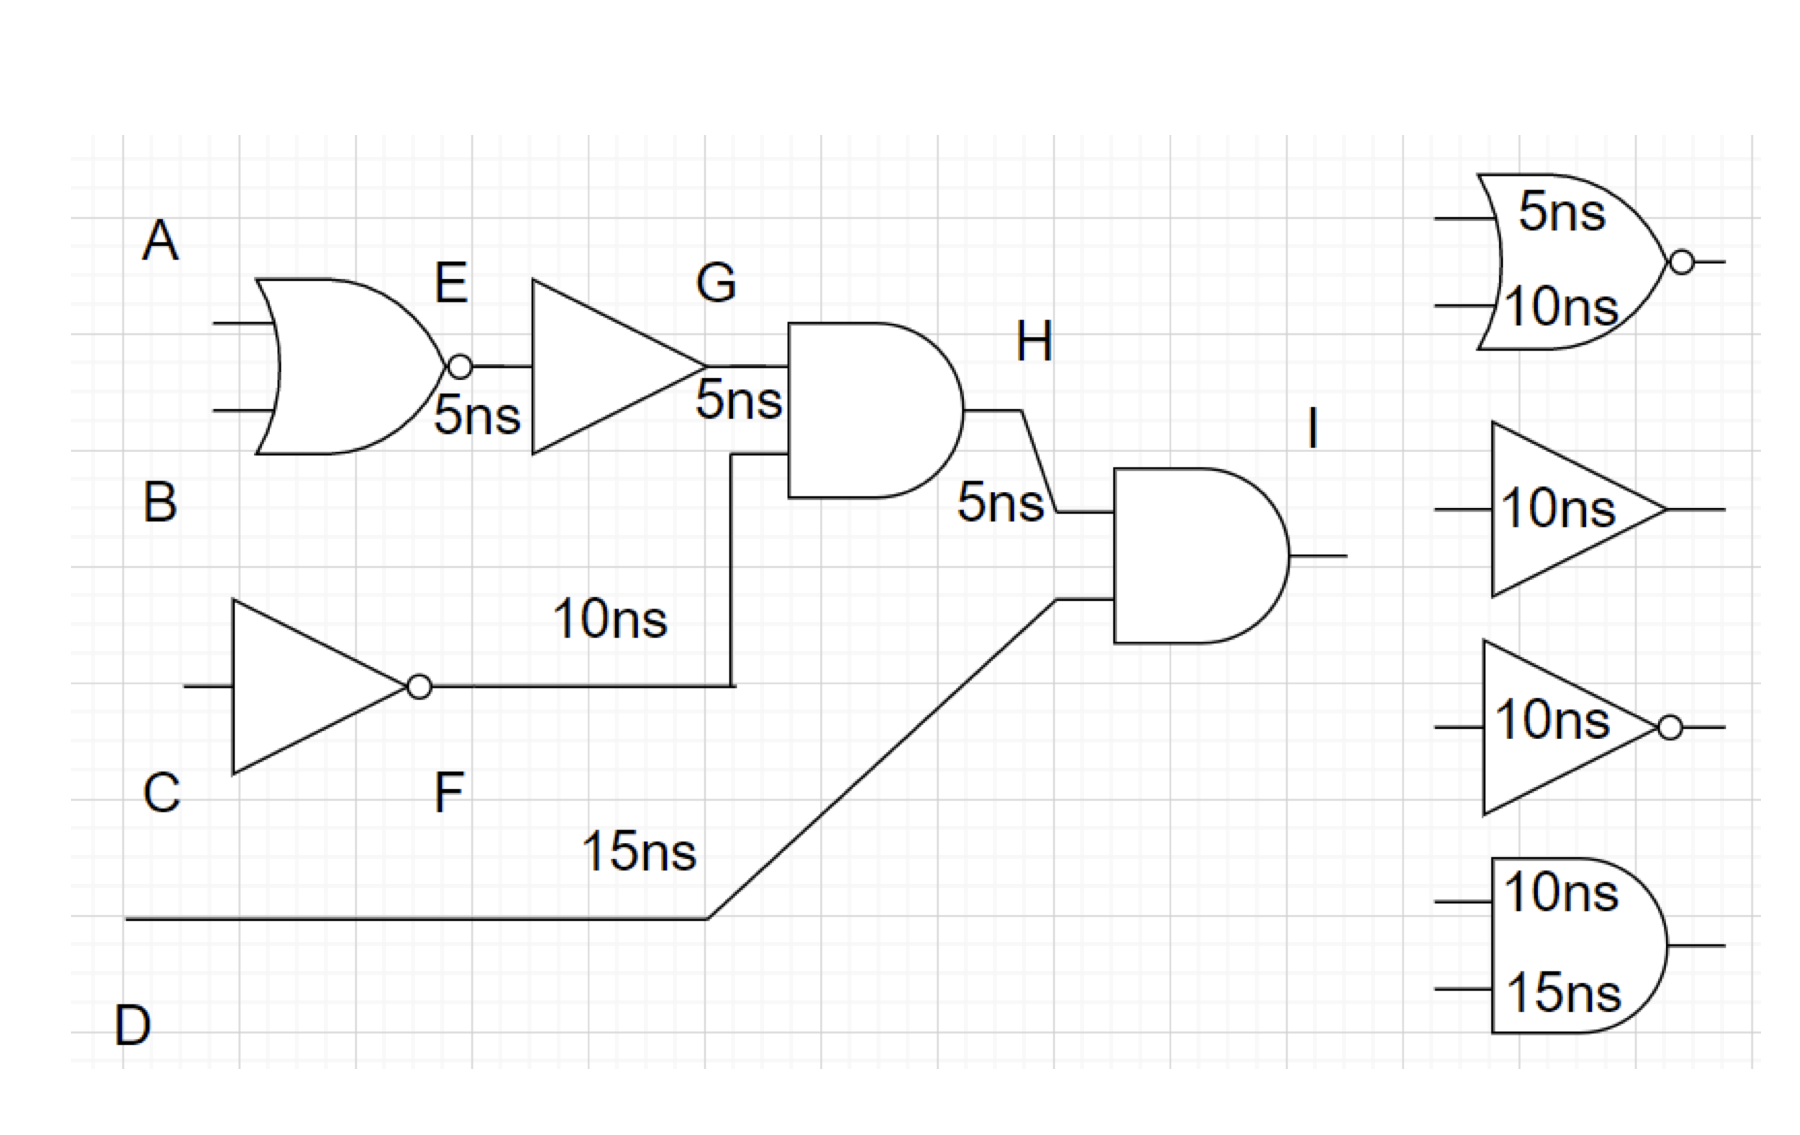
\includegraphics[width=0.56\linewidth]{problem2.png}
  \caption{题目 Figure 2：组合电路及延迟。图片裁自作业原 PDF。}
\end{figure}

图右侧标出门输入到输出的延迟，电路内部标注的是对应连线延迟。以每个字母标记处为节点，
将连线和下一级门弧的延迟相加，得到下表中的有效边权。
\begin{center}\small
\begin{tabular}{lrrrrrrrr}
\toprule
边 & $A\to E$ & $B\to E$ & $C\to F$ & $E\to G$ & $G\to H$ & $F\to H$ & $H\to I$ & $D\to I$\\
\midrule
$d$ / ns & 5 & 10 & 10 & $5+10$ & $5+10$ & $10+15$ & $5+10$ & $15+15$\\
\bottomrule
\end{tabular}
\end{center}
由 $\AT(A)=\AT(B)=\AT(C)=\AT(D)=0$ 前向传播：
\begin{align*}
\AT(E)&=\max(0+5,0+10)=10, & \AT(F)&=0+10=10,\\
\AT(G)&=10+15=25, & \AT(H)&=\max(25+15,10+25)=40,\\
\AT(I)&=\max(40+15,0+30)=55.
\end{align*}
由 $\RAT(I)=50$ 反向传播，得
$\RAT(H)=35$、$\RAT(D)=20$、$\RAT(G)=20$、$\RAT(F)=10$、
$\RAT(E)=5$，再传播到主输入。
\begin{center}\small
\begin{tabular}{crrr}
\toprule
节点 & AT / ns & RAT / ns & slack / ns\\
\midrule
$A$ & 0 & 0 & 0\\
$B$ & 0 & $-5$ & $-5$\\
$C$ & 0 & 0 & 0\\
$D$ & 0 & 20 & 20\\
$E$ & 10 & 5 & $-5$\\
$F$ & 10 & 10 & 0\\
$G$ & 25 & 20 & $-5$\\
$H$ & 40 & 35 & $-5$\\
$I$ & 55 & 50 & $-5$\\
\bottomrule
\end{tabular}
\end{center}
关键路径为 $B\to E\to G\to H\to I$，总延迟 $10+15+15+15=55$ ns，
相对 50 ns 的约束违反 5 ns。

\clearpage
\section{Problem 3：Setup analysis before CPPR}
\begin{figure}[H]
  \centering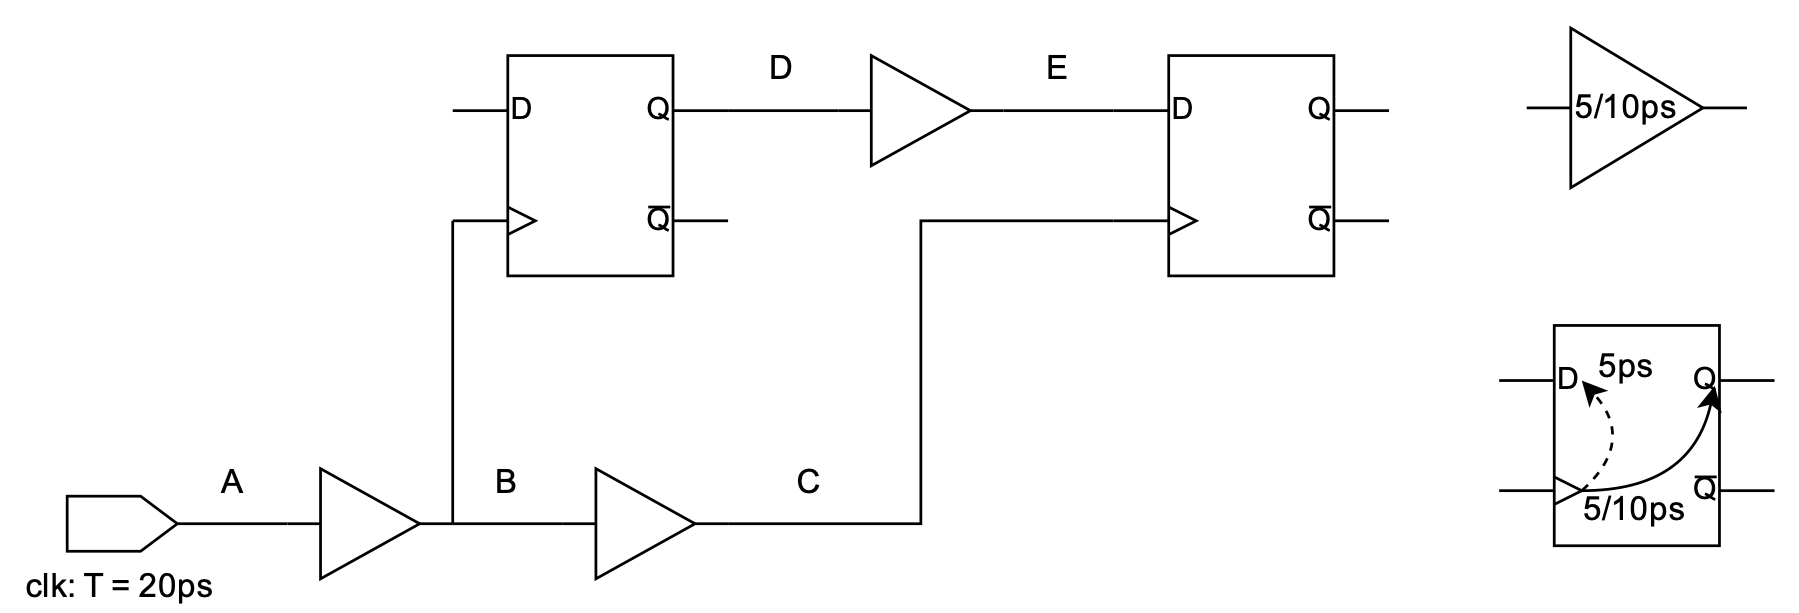
\includegraphics[width=0.80\linewidth]{problem3.png}
  \caption{题目 Figure 3：同相时钟树及寄存器间数据路径。}
\end{figure}

$A$ 是时钟根节点，$B$ 是第一级时钟缓冲器输出及发射 FF 的时钟端，
$C$ 是第二级时钟缓冲器输出及捕获 FF 的时钟端。
图中 $D$ 是发射 FF 的数据输出，$E$ 是捕获 FF 的数据输入。
每个缓冲器及 FF 的 clock-to-Q 延迟均为 early/late $=5/10$ ps；线延迟为零。
\begin{center}
\begin{tabular}{clrr}
\toprule
节点 & early AT / ps & late AT / ps\\
\midrule
$A$ & 0 & 0\\
$B$ & 5 & 10\\
$C$ & 10 & 20\\
$D$ & 10 & 20\\
$E$ & 15 & 30\\
\bottomrule
\end{tabular}
\end{center}
capture edge到达 $C$ 的绝对 early/late 时刻为 $20+10=30$ ps 和 $20+20=40$ ps。

setup 检查使用 late 数据 AT、early capture edge 和 $t_{\mathrm{setup}}=5$ ps：
\[
\RAT(E)=T+\AT_{\mathrm{early}}(C)-t_{\mathrm{setup}}=20+10-5=25\ \mathrm{ps},
\]
\[
\RAT(D)=\RAT(E)-d^{\mathrm{late}}_{D\to E}=25-10=15\ \mathrm{ps}.
\]
于是 $\slack(D)=15-20=-5$ ps，$\slack(E)=25-30=-5$ ps。
两者均违反 setup 约束。

\section{Problem 4：Inverted capture clock}
将 $B\to C$ 的缓冲器换成反相器后，按照题意，捕获可用时间改为半周期
$T/2=10$ ps。时钟路径 early 延迟仍为 $5+5=10$ ps，故
\[
\RAT(E)=T/2+\AT_{\mathrm{early}}(C)-t_{\mathrm{setup}}=10+10-5=15\ \mathrm{ps}.
\]
数据路径未变，$\AT_{\mathrm{late}}(E)=30$ ps；相应的 CPPR 前 slack 为 $-15$ ps。

\clearpage
\section{Problem 5：Setup timing with CPPR}
\subsection{模型与数据来源}
输入使用 OpenROAD 的 \code{src/rsz/test/gcd_asap7_cts.v}、对应 SDC 和 ASAP7 FF 工艺角库。
OpenROAD 提交为 \code{41a28926b92c5c20f41f89e90222a95a820384d2}；
其 OpenSTA 版本为 3.1.0，提交为 \code{779d47250b65b121ad22c70eb42e242292f9babf}。
使用提供的 \code{run_hw2.py} 原样读取标称弧延迟，由自行实现的 \code{sta.py}
完成全部时序传播、CPPR 和路径回溯。

本题设定为 $T=0.28$ ns，early/late cell-delay derate 分别为 0.9/1.1，
setup check 不加 derate；线延迟、时钟源延迟与 uncertainty 均为零。
只处理一棵非反相时钟树、上升沿 FF 和整周期 setup。FF 的 Q/QN 是数据起点、D 是端点，
不添加 D 到 Q 的数据边。数据 rise/fall 弧合并为最大 late 延迟，时钟仅保留 rise-to-rise 弧。
PI/tie 起点 AT 为零，且没有 CPPR credit。
实际读入 1221 个数据节点、46 个时钟节点、70 个数据起点（包括 FF 输出、PI 与 tie）、35 个 FF 数据端点，共有 1199 个可达起点--端点对。CPPR 后共有 10 个端点的最坏起点发生变化。


\subsection{七个函数及递推关系}
\begin{center}\small
\begin{tabularx}{\linewidth}{P{4.15cm}X}
\toprule
函数 & 实现要点\\
\midrule
\code{topological_order} & Kahn 入度队列，处理所有数据节点；若输出节点数不足则报告环。\\
\code{propagate_clock} & 从根开始按父子关系累加 early/late 边延迟，不依赖节点 ID 顺序。\\
\code{propagate_arrival} & 对每个起点单独做最大 AT 传播，记录前驱；不可达值为 \code{None}。\\
\code{propagate_required} & 初始化所有 FF 端点约束后逆拓扑取最小值；无约束节点为 $+\infty$。\\
\code{compute_cppr} & 沿父指针找到两条根路径，比较公共前缀，返回 credit 和最后公共引脚名。\\
\code{summarize_endpoints} & 枚举可达起点--端点对，修正前后分别选最小 slack，再统计 WNS/TNS。\\
\code{trace_critical_path} & 在所选起点的前驱表中从端点反向回溯，再反转得到数据路径。\\
\bottomrule
\end{tabularx}
\end{center}
对于起点 $s$，只初始化该起点：
\[
\AT_s(s)=t_{cq}(s)+L(c_s),\qquad
\AT_s(v)=\max_{u\to v}\{\AT_s(u)+d^{\mathrm{late}}_{uv}\}.
\]
其中 PI/tie 没有 $c_s$，起点初始化为零。不能先合并所有起点的 AT：
不同起点到同一端点共享的时钟路径不同，最大 AT 的起点可能在 CPPR 后不再最坏。
相同 AT 的候选前驱选择较小 ID；最终 slack 相同则先按起点 ID、再按端点 ID 排序。

设 $E(c_e)$ 为捕获时钟的 early 到达时间，$P_s,P_e$ 为根到发射/捕获时钟引脚的路径，则
\begin{align*}
 R_0(e)&=T+E(c_e)-t_{\mathrm{setup}}(e),\\
 \Delta(s,e)&=\sum_{a\in\operatorname{prefix}(P_s,P_e)}(d_a^{\mathrm{late}}-d_a^{\mathrm{early}}),\\
 R_1(s,e)&=R_0(e)+\Delta(s,e),\qquad
 S_1(s,e)=R_1(s,e)-\AT_s(e).
\end{align*}
\code{propagate_required} 返回的是基准 $R_0$ 的反向传播；CPPR 后 RAT 与起点有关，
因此修正保存在每个 pair 中，不合并成单个节点 RAT。

\clearpage
\subsection{端点统计、复杂度与运行结果}
每个端点分别计算 $S_k(e)=\min_s S_k(s,e)$，其中 $k=0,1$ 分别代表修正前后。
本报告采用以下 WNS/TNS 定义：
\[
 \mathrm{WNS}_k=\min\!\left(0,\min_e S_k(e)\right),\qquad
 \mathrm{TNS}_k=\sum_e\min(0,S_k(e)).
\]
TNS 对每个端点只计一次；即使没有违反，仍可记录最小 slack 所对应的路径。

设数据节点、数据边、起点、端点、时钟节点数分别为 $N,M,S,K,C$，时钟树高度为 $h$。
拓扑排序、单次 RAT 传播均为 $O(N+M)$；时钟传播为 $O(C)$；逐起点 AT 传播为
$O(S(N+M))$，AT 与前驱表空间为 $O(SN)$；本实现逐 pair 沿父指针求 CPPR，
汇总时间为 $O(SKh)$，只输出可达 pair。对于本实验规模，无需额外的 LCA 预处理。

\begin{center}\small
\begin{tabular}{lrr}
\toprule
指标 & CPPR 前 & CPPR 后 \\
\midrule
WNS / ns & -0.012235756 & -0.008608215 \\
TNS / ns & -0.056881131 & -0.019221813 \\
关键路径 AT / ns & 0.319313124 & 0.319313124 \\
关键路径 RAT / ns & 0.307077368 & 0.310704909 \\
负 slack 端点数 & 9 & 3 \\
\bottomrule
\end{tabular}
\end{center}

CPPR 提高了 slack，但仍有 3 个负 slack 端点，故在该标量模型下 0.28 ns 周期仍未满足。
全局最坏 pair 的公共引脚是 \code{clkbuf_0_clk/Y}，修正量为
$0.003627541496$ ns；WNS 的改善量与该值一致。

CPPR 前：\code{dpath.a_reg.out[13]$_DFFE_PP_/QN} $\longrightarrow$ \code{dpath.a_reg.out[7]$_DFFE_PP_/D}。

CPPR 后：\code{dpath.a_reg.out[13]$_DFFE_PP_/QN} $\longrightarrow$ \code{dpath.a_reg.out[7]$_DFFE_PP_/D}。

两次全局最坏路径在本例中相同，完整的数据引脚序列如下：
\begin{lstlisting}[style=script,language={},numbers=none]
dpath.a_reg.out[13]$_DFFE_PP_/QN
 -> _361_/A -> _361_/Y
 -> _563_/B -> _563_/SN
 -> _324_/B -> _324_/Y
 -> _325_/A2 -> _325_/Y
 -> _326_/A2 -> _326_/Y
 -> _327_/B -> _327_/Y
 -> _328_/B1 -> _328_/Y
 -> _366_/A -> _366_/Y
 -> _477_/A -> _477_/Y
 -> _480_/B1 -> _480_/Y
 -> dpath.a_reg.out[7]$_DFFE_PP_/D
\end{lstlisting}

这里“路径相同”只针对全局最坏 pair；其他端点仍须独立重选起点。
\code{result.json} 中保存前后完整关键路径，\code{node_timing.json} 保存逐起点的
所有节点 AT/前驱、时钟 AT、拓扑顺序及 CPPR 前节点 RAT。

\clearpage
\subsection{最坏起点改变的实际端点}
端点为 \code{dpath.b_reg.out[5]$_DFFE_PP_/D}，记两个候选起点为：
\begin{itemize}
\item L1：\code{dpath.a_reg.out[7]$_DFFE_PP_/QN}。
\item L2：\code{dpath.a_reg.out[9]$_DFFE_PP_/QN}。
\end{itemize}
\begin{center}\small
\begin{tabular}{lrrrr}
\toprule
起点 & AT / ns & slack 前 / ns & CPPR / ns & slack 后 / ns \\
\midrule
L1 & 0.312791381 & -0.005704594 & 0.009021508 & 0.003316913 \\
L2 & 0.309360046 & -0.002273259 & 0.003627541 & 0.001354282 \\
\bottomrule
\end{tabular}
\end{center}
L1 的公共时钟引脚为 \code{clkbuf_2_0__f_clk/Y}；L2 的公共时钟引脚为 \code{clkbuf_0_clk/Y}。

修正前，L1 的 slack 更小；修正后，L1 共享的时钟前缀较长，得到更大的 credit，
最坏起点转为 L2。该端点的最坏 slack 从 $-0.005704594$ ns 变为 $+0.001354282$ ns。
若只修正原来的 L1 并继续把它作为最坏起点，会误报为 $+0.003316913$ ns，
高估该端点的裕量。这验证了逐起点保留 AT 并重新选取最坏路径的必要性。

\subsection{独立运行 OpenSTA 比较 CPPR}
使用 \code{compare_opensta.py} 另起 OpenSTA 进程，读入相同网表和库。
读完原 SDC 后执行 \code{set_cmd_units -time ns} 并将时钟周期重设为 0.28 ns，
避免将 ASAP7 的 ps 库单位直接误作 ns。原 SDC 的 I/O 约束予以保留。
采用传播时钟及 on-chip variation 分析，核心对照设置为：
\begin{lstlisting}[style=script,language={},numbers=none]
set_timing_derate -early -cell_delay 0.9
set_timing_derate -late -cell_delay 1.1
sta::set_crpr_mode same_transition
\end{lstlisting}
脚本将 \code{sta::set_crpr_enabled} 分别设为 0 和 1，固定发射 FF 时钟引脚、
数据输出引脚和接收 D 引脚，输出
\code{full_clock_expanded} 文本与 JSON；比较实际报告中的 credit，同时检查
两条原生时钟路径的最后公共引脚与本实现一致。
所比较的三对路径为：
\begin{itemize}
\item P1：\code{dpath.a_reg.out[13]$_DFFE_PP_/QN} $\to$ \code{dpath.a_reg.out[7]$_DFFE_PP_/D}。
\item P2：\code{dpath.a_reg.out[7]$_DFFE_PP_/QN} $\to$ \code{dpath.b_reg.out[5]$_DFFE_PP_/D}。
\item P3：\code{dpath.a_reg.out[9]$_DFFE_PP_/QN} $\to$ \code{dpath.b_reg.out[5]$_DFFE_PP_/D}。
\end{itemize}
\begin{center}\small
\begin{tabular}{lrrr}
\toprule
路径 & 本实现 CPPR / ns & OpenSTA CPPR / ns & 绝对误差 / ns \\
\midrule
P1 & 0.003627541 & 0.003627542 & 5.04e-10 \\
P2 & 0.009021508 & 0.009021506 & 1.67e-09 \\
P3 & 0.003627541 & 0.003627542 & 5.04e-10 \\
\bottomrule
\end{tabular}
\end{center}

三对路径均通过 $2\times10^{-8}$ ns 的绝对误差门限，最大实际误差约为
$1.67\times10^{-9}$ ns。浮点计算与文本舍入可解释此量级的差异。
OpenSTA 原生 slack 与本实现不同：本题将各级数据 rise/fall 弧独立取最大，
而 OpenSTA 保留跃迁一致性，且使用原生 SDC 约束。故此处验证的是 CPPR credit，
不能用原生绝对 slack 替代本题的计算结果。

\clearpage
\subsection{完整输出与验证}
\code{run_gcd/pairs.csv} 和 \code{run_gcd/result.json} 提供全部 1199 个可达
起点--端点对的 AT、修正前后 RAT/slack、CPPR credit 与公共时钟引脚，
\code{run_gcd/endpoints.csv} 提供全部 35 个端点修正前后的最坏起点及 slack。
正文选取代表性 pair 展示，完整逐对明细随源码一同提交。

\code{test_sta.py} 的 14 项测试全部通过，覆盖非拓扑 ID、组合环检测、时钟树异常、
共享根/共享分支/同叶/祖先时钟引脚、PI 零 credit、不可达节点、相等 AT 的前驱选择、
多端点 RAT、CPPR 后最坏起点重选、TNS 去重、正 slack、回溯环检测及 Problem 2 手算表。
其中随机测试固定种子为学号 2300012831，对 100 个小型 DAG 穷举路径，独立核对
逐起点 AT、RAT、回溯路径和端点汇总。

此外，真实 gcd 输入已通过提供的 runner 完整运行，输出 JSON 不含非有限数值；
OpenSTA 独立对照的三对 credit 和公共引脚全部匹配。
输入库读取过程中出现上游 Liberty 的 \code{Warning 1212}、物理 TAPCELL 黑盒警告，
以及原 SDC 对时钟输入设置 input delay 的警告，均记录于日志。
这些警告来自原始输入；本实验未改动网表、库、SDC 或 OpenSTA 源码。

在 \code{HW2_STA} 目录运行以下命令即可复现（环境变量按本机工具位置设置）：
\begin{lstlisting}[style=script,language={},numbers=none]
python3 -m unittest -v
python3 run_hw2.py --openroad-root "$OPENROAD_ROOT" --sta "$STA"
python3 compare_opensta.py --openroad-root "$OPENROAD_ROOT" --sta "$STA"
python3 export_report.py
\end{lstlisting}
README 给出环境变量的准确路径、完整参数与报告编译命令。
\code{run_hw2.py} 保持作业提供的版本；其默认结果完全由本实现的七个函数计算。

\section*{附录：AI 使用记录}
本次使用 Codex 辅助读取作业要求和电路图、推导 Problems 1--4、实现 Problem 5
的七个函数，并编写单元测试、OpenSTA 对照脚本、结果导出脚本及 README。
AI 还协助在本机编译 OpenSTA、按要求安装仅含 XeTeX 引擎的最小 TeX 环境，
整理中文报告、裁取原题插图并执行 XeLaTeX 编译。

报告中的实验数字来自实际运行生成的 JSON 和 OpenSTA 报告，测试结论来自实际执行日志。
程序与报告仍受本题的简化假设限制，不涉及 hold 分析、多时钟域、反相时钟树、
多周期例外、寄生 RC 提取或真实路径可敏化性分析。

\end{document}
